% Mục 5.2: Bài toán hồi quy tuyến tính bội.
% Số liệu lấy từ generated/regression_*.tex, sinh bởi scripts/reports/report_regression.py.
% Dùng nguyên bộ dữ liệu cuối của Mục 3 (loại các dòng khuyết xung nhịp lõi);
% mục này không sửa hay tạo thêm dữ liệu.
% Cần: booktabs, graphicx, listings, amsmath; macro \Reg... từ regression_numbers.tex.
% Khi ghép vào báo cáo chính: thêm hai tài liệu cameron2015 và duan1983
% (xem preview_section5_regression.tex).

\subsection{Bài toán hồi quy tuyến tính}
\label{sec:regression}

\subsubsection{Đề xuất phương pháp}
\label{sec:reg-method}

Phân tích phương sai ở Mục~\ref{sec:anova} cho thấy công suất tối đa khác nhau rõ giữa các nhóm
loại bộ nhớ, nhưng chưa tách được tác động riêng của từng thông số phần cứng khi các yếu tố
này cùng thay đổi theo thế hệ sản phẩm. Để định lượng đồng thời mối liên hệ giữa công suất tiêu
thụ tối đa và các đặc trưng kỹ thuật của GPU rời, ta xây dựng mô hình hồi quy tuyến tính bội
trên thang logarit tự nhiên.

\begin{center}
\fbox{\parbox{0.92\linewidth}{\textbf{Bài toán.} Với mức ý nghĩa $\alpha = \RegAlpha$ (độ tin
cậy $\RegConfidence\%$), các thông số kỹ thuật gồm băng thông bộ nhớ, xung nhịp lõi, kích thước
tiến trình chế tạo và dung lượng bộ nhớ có đồng thời liên hệ có ý nghĩa thống kê với công suất
tối đa ($\ln P$) sau khi kiểm soát hãng sản xuất và phân khúc thiết bị hay không?}}
\end{center}

Từ \RegRowsInput{} dòng dữ liệu cuối của Mục~3 (\texttt{gpus\_analysis}), mô hình loại
\RegRowsExcluded{} dòng chỉ bị khuyết xung nhịp lõi (\texttt{core\_speed\_mhz}) và giữ lại
$n = \RegN{}$ quan sát đầy đủ thuộc \RegClusters{} nhãn kiến trúc (\texttt{architecture}) khác
nhau. Biến phụ thuộc là $z_i = \ln P_i$, với $P_i$ là công suất tối đa (\texttt{max\_power\_w},
đơn vị W). Các biến giải thích đưa vào mô hình gồm:
\begin{itemize}
  \item Bốn biến kỹ thuật: $\ln B_i$ với $B_i$ là băng thông bộ nhớ (\texttt{memory\_bandwidth\_gb\_s},
    GB/s); $\ln F_i$ với $F_i$ là xung nhịp lõi (\texttt{core\_speed\_mhz}, MHz); $L_i$ là kích
    thước tiến trình chế tạo (\texttt{process\_nm}, nm); và $\ln M_i$ với $M_i$ là dung lượng
    bộ nhớ quy đổi về GB (\texttt{memory\_mb / 1024}).
  \item Các biến phân loại kiểm soát: hai biến giả hãng sản xuất $D_{i,\mathrm{AMD}}$ và
    $D_{i,\mathrm{ATI}}$ (lấy \texttt{Nvidia} làm nhóm tham chiếu), cùng biến giả phân khúc
    $N_i = 1$ nếu là GPU \texttt{Laptop} và $N_i = 0$ nếu là \texttt{Desktop}.
\end{itemize}

Tương tự hạn chế đã nêu ở Mục~\ref{sec:anova-method}, nhiều card đồ họa trong dữ liệu là các
phiên bản thương mại khác nhau của cùng một kiến trúc chip nên không độc lập hoàn toàn. Do đó,
suy diễn thống kê chính trong mục này sử dụng ma trận hiệp phương sai vững theo cụm
(\textit{cluster-robust}, hiệu chỉnh hữu hạn mẫu CR1) phân nhóm theo \RegClusters{} kiến trúc
\cite{cameron2015}, với bậc tự do phân phối $t$ là $\RegClusters - 1 = \RegPrimaryDfTwo$.

\subsubsection{Mô hình}
\label{sec:reg-model}

Mô hình hồi quy log--tuyến tính bội có dạng:
\begin{equation}
  z_i = \ln P_i = \beta_0 + \beta_1 \ln B_i + \beta_2 \ln F_i + \beta_3 L_i + \beta_4 \ln M_i
        + \gamma_{\mathrm{AMD}} D_{i,\mathrm{AMD}} + \gamma_{\mathrm{ATI}} D_{i,\mathrm{ATI}}
        + \delta N_i + \varepsilon_i.
  \label{eq:reg-model}
\end{equation}

Để kiểm định vai trò đồng thời của bốn thông số kỹ thuật sau khi kiểm soát hãng sản xuất và
loại thiết bị, ta đặt cặp giả thuyết:
\[
  H_0: \beta_1 = \beta_2 = \beta_3 = \beta_4 = 0, \qquad
  H_1: \text{tồn tại ít nhất một } \beta_j \ne 0 \quad (j \in \{1, 2, 3, 4\}).
\]

Kết quả ước lượng bình phương tối thiểu (OLS) kèm ba loại sai số chuẩn (cổ điển OLS, vững
phương sai thay đổi HC3 và vững theo cụm kiến trúc) được trình bày ở Bảng~\ref{tab:reg-coef}.
Thay các hệ số ước lượng vào phương trình~\eqref{eq:reg-model}, ta thu được mô hình thực nghiệm:
\begin{align*}
  \widehat{\ln P_i} ={} & 1{,}173 + 0{,}695 \ln B_i - 0{,}047 \ln F_i + 0{,}018 L_i + 0{,}099 \ln M_i \\
                        & - 0{,}024 D_{i,\mathrm{AMD}} - 0{,}129 D_{i,\mathrm{ATI}} - 0{,}500 N_i.
\end{align*}

\begin{table}[htbp]
  \centering
  \caption{Kết quả ước lượng hồi quy bội cho $\ln P$ ($n = \RegN$, \RegClusters{} cụm kiến trúc)}
  \label{tab:reg-coef}
  \small
  \resizebox{\linewidth}{!}{%
  \begin{tabular}{l r r r r c r}
    \toprule
    \textbf{Biến / Hệ số} & \textbf{Ước lượng} & \textbf{SE (OLS)} & \textbf{SE (HC3)}
      & \textbf{SE (Cụm)} & \textbf{KTC \RegConfidence\% (Cụm)} & \textbf{\boldmath$p$ (Cụm)} \\
    \midrule
    \csname @@input\endcsname generated/regression_coef_table.tex
    \bottomrule
  \end{tabular}%
  }
\end{table}

Mô hình đạt hệ số xác định $R^2 = \RegRSquared$ và $R^2_{\mathrm{adj}} = \RegAdjRSquared$ trên
thang $\ln P$. Kiểm định Wald đồng thời bốn hệ số kỹ thuật theo sai số chuẩn cụm cho
$F(\RegPrimaryDfOne;\ \RegPrimaryDfTwo) = \RegPrimaryF$ với $p = \RegPrimaryP \le \RegAlpha$,
nên ta bác bỏ $H_0$: nhóm thông số kỹ thuật có liên hệ có ý nghĩa thống kê rất mạnh với công
suất GPU.

Bảng~\ref{tab:reg-coef} cũng cho thấy sai số chuẩn cụm lớn gấp khoảng $2$ đến $2{,}5$ lần sai
số chuẩn OLS và HC3, phản ánh rõ sự tương quan giữa các card cùng kiến trúc. Bảng~\ref{tab:reg-effects}
quy đổi từng hệ số sang tác động phần trăm chính xác lên trung bình hình học có điều kiện
$\exp\{\mathrm{E}(\ln P \mid \mathbf{x})\}$ khi giữ các biến còn lại cố định:
\begin{itemize}
  \item \textbf{Băng thông bộ nhớ ($\ln B$):} Là yếu tố chi phối mạnh nhất ($\hat{\beta}_1 = 0{,}695$,
    $p = 7{,}25 \cdot 10^{-83}$). Khi băng thông tăng $1\%$, trung bình hình học công suất tăng
    $100[(1{,}01)^{\hat{\beta}_1} - 1] = 0{,}694\%$.
  \item \textbf{Kích thước tiến trình ($L$):} Có ý nghĩa thống kê cao ($\hat{\beta}_3 = 0{,}018$,
    $p = 2{,}36 \cdot 10^{-10}$). Với cùng băng thông, xung nhịp và dung lượng bộ nhớ, tiến trình
    lớn hơn $1\text{ nm}$ đi kèm công suất cao hơn $100[\exp(\hat{\beta}_3) - 1] = 1{,}840\%$, phản
    ánh hiệu quả năng lượng cải thiện ở các tiến trình thu nhỏ.
  \item \textbf{Dung lượng bộ nhớ ($\ln M$):} Có ý nghĩa thống kê ở mức $\alpha = \RegAlpha$
    ($\hat{\beta}_4 = 0{,}099$, $p = 0{,}0045$); tăng $1\%$ dung lượng VRAM tương ứng mức tăng
    $0{,}098\%$ công suất.
  \item \textbf{Xung nhịp lõi ($\ln F$):} Không có ý nghĩa thống kê ($\hat{\beta}_2 = -0{,}047$,
    $p = 0{,}6628$) sau khi đã kiểm soát băng thông, tiến trình và dung lượng bộ nhớ, do xung nhịp
    cao thường xuất hiện ở các thế hệ chip mới dùng tiến trình nhỏ hơn.
  \item \textbf{Phân khúc thiết bị và hãng sản xuất:} Ở cùng thông số kỹ thuật, GPU
    \texttt{Laptop} có trung bình hình học công suất thấp hơn \texttt{Desktop} là $39{,}333\%$
    ($\hat{\delta} = -0{,}500$, $p = 4{,}20 \cdot 10^{-17}$). Ngược lại, chênh lệch giữa
    \texttt{AMD} ($p = 0{,}4904$) và \texttt{ATI} ($p = 0{,}0296 > \RegAlpha$) so với
    \texttt{Nvidia} đều không đạt mức ý nghĩa $\RegAlpha$ sau khi điều chỉnh thông số kỹ thuật.
\end{itemize}

\begin{table}[htbp]
  \centering
  \caption{Tác động phần trăm chính xác lên trung bình hình học có điều kiện của công suất}
  \label{tab:reg-effects}
  \small
  \begin{tabular}{l r l}
    \toprule
    \textbf{Biến / Hệ số} & \textbf{Tác động (\%)}
      & \textbf{Cơ sở so sánh (giữ các biến khác cố định)} \\
    \midrule
    \csname @@input\endcsname generated/regression_effects_table.tex
    \bottomrule
  \end{tabular}
\end{table}

\subsubsection{Kiểm tra giả định mô hình hồi quy bội}
\label{sec:reg-diagnostics}

Để đánh giá độ tin cậy của mô hình tuyến tính cổ điển và lý giải việc sử dụng sai số chuẩn vững,
ta kiểm tra đa cộng tuyến thông qua hệ số phóng đại phương sai $\mathrm{VIF}_j$
(Bảng~\ref{tab:reg-vif}) cùng các kiểm định giả định trên phần dư OLS (Bảng~\ref{tab:reg-diag}
và Hình~\ref{fig:reg-diag}).

\begin{table}[htbp]
  \centering
  \begin{minipage}[t]{0.40\linewidth}
    \centering
    \caption{Hệ số phóng đại phương sai ($\mathrm{VIF}$)}
    \label{tab:reg-vif}
    \small
    \begin{tabular}{l r}
      \toprule
      \textbf{Biến giải thích} & \textbf{$\mathrm{VIF}_j$} \\
      \midrule
      \csname @@input\endcsname generated/regression_vif_table.tex
      \bottomrule
    \end{tabular}
  \end{minipage}
  \hfill
  \begin{minipage}[t]{0.56\linewidth}
    \centering
    \caption{Các phép kiểm định giả định phần dư OLS}
    \label{tab:reg-diag}
    \small
    \begin{tabular}{l r r}
      \toprule
      \textbf{Phép kiểm định} & \textbf{Thống kê} & \textbf{\boldmath$p$} \\
      \midrule
      \csname @@input\endcsname generated/regression_diagnostics_table.tex
      \bottomrule
    \end{tabular}
  \end{minipage}
\end{table}

\begin{itemize}
  \item \textbf{Đa cộng tuyến:} Giá trị $\mathrm{VIF}$ lớn nhất thuộc về $\ln F$ ($\RegMaxVIF$),
    tiếp theo là $L$ ($3{,}46$) và $\ln M$ ($2{,}85$). Tất cả các biến đều dưới ngưỡng cảnh báo
    $5$, cho thấy mức tương quan giữa các biến giải thích không gây mất ổn định nghiêm trọng
    cho ước lượng hệ số.
  \item \textbf{Tính tuyến tính và phương sai sai số:} Trên biểu đồ \textit{Residuals vs Fitted}
    (Hình~\ref{fig:reg-diag}, góc trên bên trái), đường làm mượt LOWESS bám sát trục $0$, ủng hộ
    dạng hàm tuyến tính trên thang log. Tuy nhiên, biểu đồ \textit{Scale-Location} cùng kiểm
    định Breusch--Pagan ($\mathrm{LM} = 258{,}671$, $p = 3{,}95 \cdot 10^{-52}$) và kiểm định
    White ($\mathrm{LM} = 360{,}689$, $p = 6{,}38 \cdot 10^{-59}$) đều bác bỏ mạnh giả định
    phương sai đồng nhất. Điều này khẳng định việc thay thế sai số chuẩn OLS bằng sai số chuẩn
    vững theo cụm là cần thiết.
  \item \textbf{Phân phối chuẩn và điểm ảnh hưởng:} Kiểm định Shapiro--Wilk bác bỏ phân phối
    chuẩn chính xác của phần dư ($W = 0{,}974$, $p = 1{,}22 \cdot 10^{-17}$), thể hiện qua hai
    đuôi lệch khỏi đường tham chiếu trên đồ thị Q--Q (Hình~\ref{fig:reg-diag}, góc trên bên phải),
    trong khi phần thân trung tâm vẫn bám khá sát đường thẳng. Với cỡ mẫu lớn ($n = \RegN$,
    \RegClusters{} cụm), suy diễn dựa trên phân phối tiệm cận của ước lượng cụm không đòi hỏi
    sai số phải chuẩn tuyệt đối \cite{cameron2015}. Trên đồ thị \textit{Residuals vs Leverage},
    các quan sát vượt đường đồng mức Cook $D = 4/n$ chỉ được dùng để nhận diện các cấu hình đặc
    thù chứ không tự động loại bỏ khỏi dữ liệu.
\end{itemize}

\begin{figure}[htbp]
  \centering
  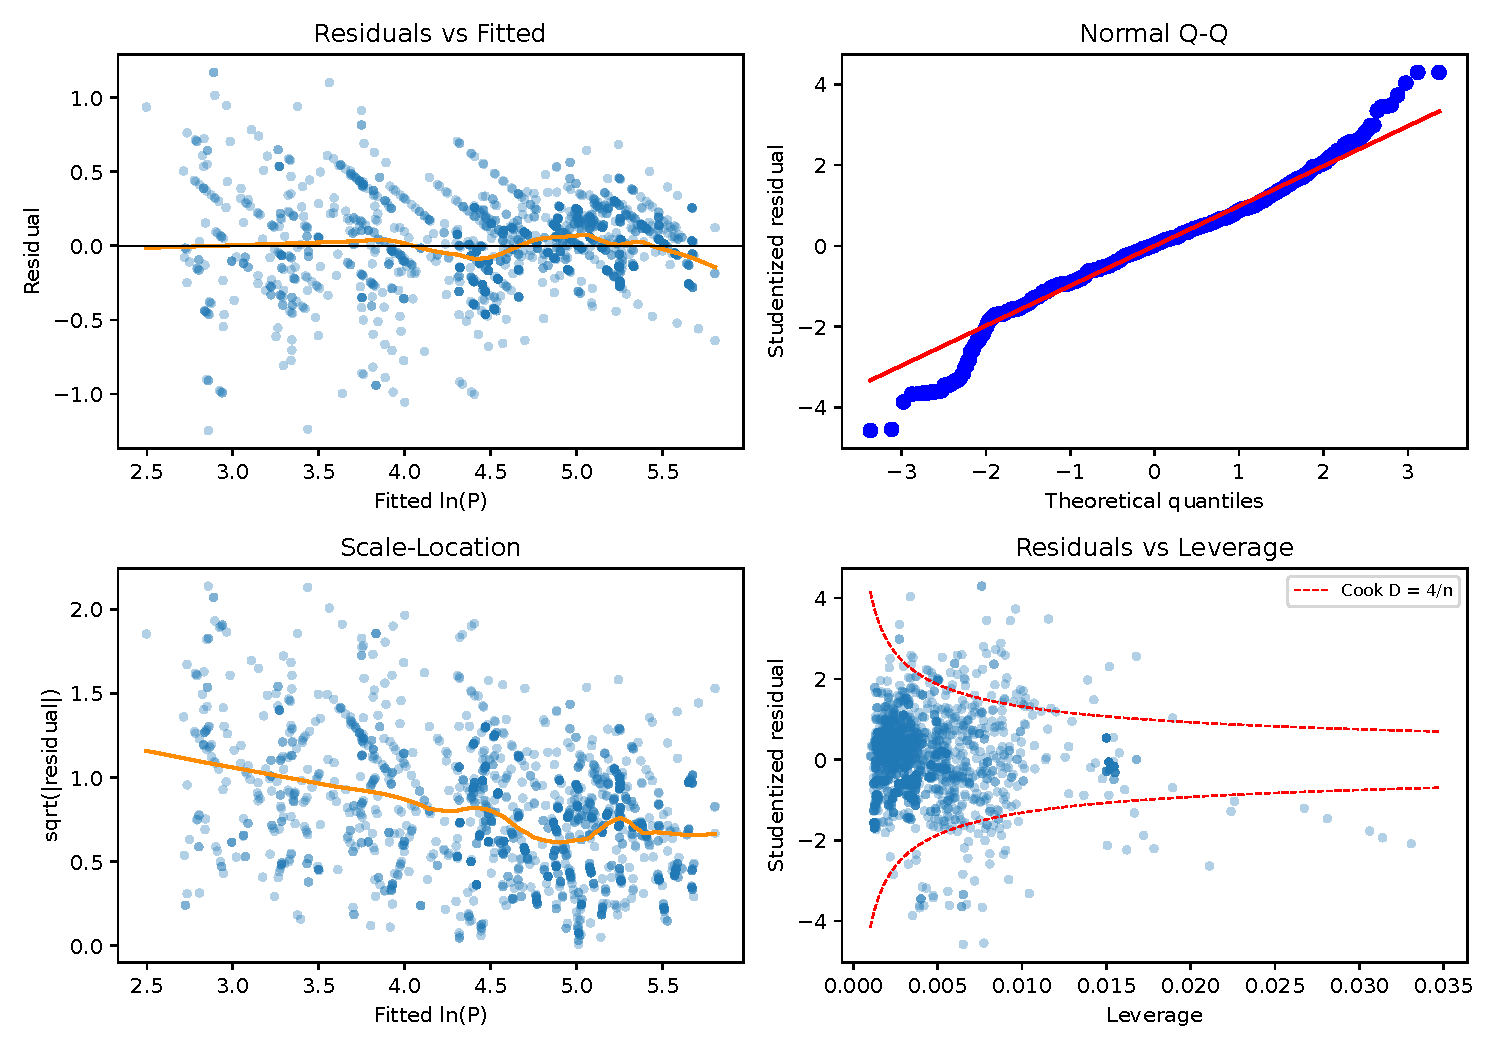
\includegraphics[width=0.92\linewidth]{generated/regression_diagnostics.pdf}
  \caption{Bộ bốn đồ thị chẩn đoán phần dư mô hình hồi quy bội: phần dư theo giá trị khớp,
    đồ thị Q--Q chuẩn, đồ thị Scale-Location và phần dư chuẩn hóa theo đòn bẩy kèm đường đồng
    mức Cook $D = 4/n$.}
  \label{fig:reg-diag}
\end{figure}

Các lệnh Python thực hiện ước lượng vững, kiểm định đồng thời và chẩn đoán mô hình được tóm tắt
ở Đoạn code~\ref{lst:regression}.

\begin{lstlisting}[language=Python, float=htbp, columns=fixed, label={lst:regression},
  caption={Các bước ước lượng và chẩn đoán chính của Mục~\ref{sec:regression} (rút gọn từ \texttt{report\_regression.py})}]
import numpy as np
import statsmodels.api as sm
from scipy import stats
from statsmodels.stats.diagnostic import het_breuschpagan, het_white
from statsmodels.stats.outliers_influence import variance_inflation_factor

ols = sm.OLS(y, X).fit()
hc3 = ols.get_robustcov_results(cov_type="HC3", use_t=True)
clustered = ols.get_robustcov_results(
    cov_type="cluster", groups=arch_groups,
    use_correction=True, df_correction=True, use_t=True,
)
joint_wald = clustered.f_test(restriction_matrix)   # H0: 4 technical slopes = 0
vif = [variance_inflation_factor(X.to_numpy(), i) for i in range(1, X.shape[1])]
bp = het_breuschpagan(ols.resid, X)
white = het_white(ols.resid, X)
shapiro = stats.shapiro(ols.resid)
smearing_factor = np.exp(ols.resid).mean()          # Duan smearing correction
\end{lstlisting}

\subsubsection{Dự báo}
\label{sec:reg-forecast}

Để đánh giá khả năng khái quát hóa trên thang công suất gốc (W) đối với các kiến trúc GPU chưa
từng xuất hiện khi huấn luyện, ta thực hiện kiểm định chéo 5 phần (\textit{5-fold cross-validation})
chia theo từng khối kiến trúc (\texttt{architecture} không trùng lặp giữa tập huấn luyện và tập
kiểm tra). Giá trị dự báo log $\hat{z}_i$ được biến đổi ngược về thang W bằng hệ số hiệu chỉnh
Duan smearing $\hat{\phi} = \frac{1}{n_{\mathrm{train}}}\sum \exp(e_i)$ tính riêng trên từng tập
huấn luyện để tránh rò rỉ dữ liệu \cite{duan1983}:
\[
  \hat{P}_{i,\mathrm{Duan}} = \exp(\hat{z}_i)\,\hat{\phi}.
\]

Kết quả đối chiếu ngoài mẫu trên toàn bộ \RegN{} quan sát (Hình~\ref{fig:reg-cv}) đạt sai số
căn phương trung bình $\mathrm{RMSE} = \RegCVRMSE\text{ W}$, sai số tuyệt đối trung bình
$\mathrm{MAE} = \RegCVMAE\text{ W}$ và hệ số xác định trên thang W là
$R^2_{\mathrm{CV}} = \RegCVRSquaredW$.

\begin{figure}[htbp]
  \centering
  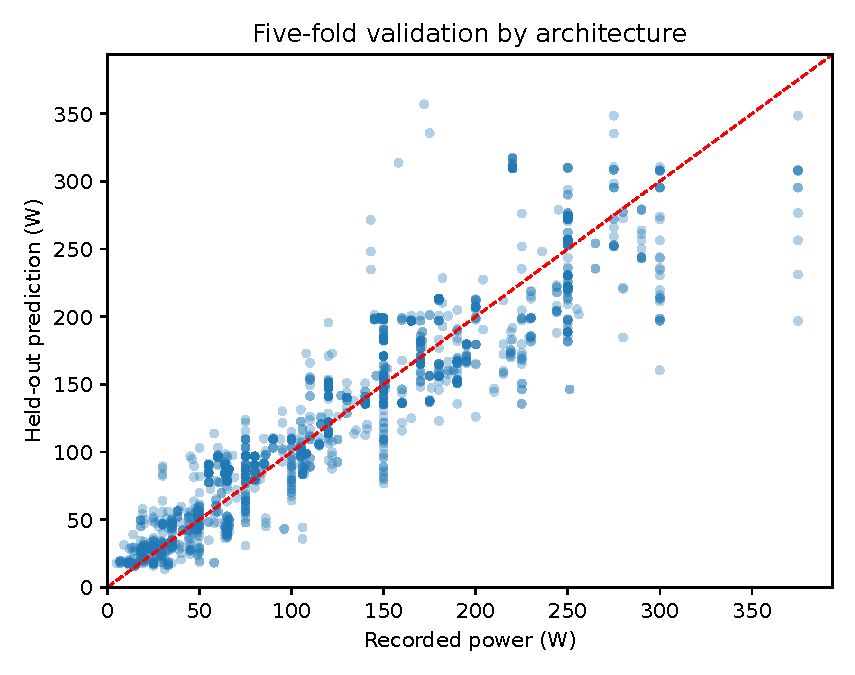
\includegraphics[width=0.68\linewidth]{generated/regression_actual_vs_pred.pdf}
  \caption{Đối chiếu công suất ghi nhận thực tế và công suất dự báo ngoài mẫu (W) từ kiểm định
    chéo 5 phần tách theo kiến trúc; đường đứt nét đỏ là đường lý tưởng $y = x$.}
  \label{fig:reg-cv}
\end{figure}

Bảng~\ref{tab:reg-forecast} minh họa kết quả ước lượng trên ba cấu hình đại diện trong mẫu tại
các mốc tứ phân vị $Q_1, Q_2, Q_3$ của băng thông bộ nhớ:
\begin{itemize}
  \item \texttt{gpu\_id = 1841} (\textit{Radeon HD 6670 MSI Dual Fan 1GB Edition}, ATI, Desktop,
    $B = 64\text{ GB/s}$, $F = 800\text{ MHz}$, $L = 40\text{ nm}$, $M = 1\text{ GB}$, công suất
    ghi nhận $66\text{ W}$);
  \item \texttt{gpu\_id = 3040} (\textit{GeForce GTX 960 MSI OC 2GB Edition}, Nvidia, Desktop,
    $B = 112{,}2\text{ GB/s}$, $F = 1176\text{ MHz}$, $L = 28\text{ nm}$, $M = 2\text{ GB}$, công
    suất ghi nhận $120\text{ W}$);
  \item \texttt{gpu\_id = 1230} (\textit{Radeon RX 480 PowerColor Red Dragon 4GB}, AMD, Desktop,
    $B = 224\text{ GB/s}$, $F = 1120\text{ MHz}$, $L = 14\text{ nm}$, $M = 4\text{ GB}$, công
    suất ghi nhận $120\text{ W}$).
\end{itemize}

\begin{table}[htbp]
  \centering
  \caption{Ước lượng công suất minh họa cho ba cấu hình tiêu biểu trong mẫu}
  \label{tab:reg-forecast}
  \begin{tabular}{r r c r}
    \toprule
    \textbf{\texttt{gpu\_id}} & \textbf{$\widehat{\mathrm{GM}}(P \mid \mathbf{x})$ (W)}
      & \textbf{KTC \RegConfidence\% cho GM (W)} & \textbf{$\hat{P}_{\mathrm{Duan}}$ (W)} \\
    \midrule
    \csname @@input\endcsname generated/regression_forecast_table.tex
    \bottomrule
  \end{tabular}
\end{table}

Cần lưu ý ba giới hạn khi sử dụng các con số ở Bảng~\ref{tab:reg-forecast}: thứ nhất, khoảng tin
cậy $\RegConfidence\%$ trong bảng bao phủ \emph{trung bình hình học có điều kiện}
$\widehat{\mathrm{GM}}(P \mid \mathbf{x}) = \exp(\mathbf{x}^\top \hat{\boldsymbol{\theta}})$
tính theo ma trận hiệp phương sai cụm, không phải khoảng dự báo cho một sản phẩm mới đơn lẻ;
thứ hai, do phương sai sai số thay đổi theo cấu hình, một hệ số hiệu chỉnh Duan tổng quát
$\hat{\phi}$ không bảo đảm ước lượng không chệch cho trung bình số học có điều kiện tại mọi
điểm; thứ ba, mô hình chỉ áp dụng trong miền thông số của bộ dữ liệu (card rời giai đoạn
2006--2017) và không nên ngoại suy cho các thế hệ GPU hiện đại ngoài miền quan sát.

\subsubsection{Kết luận}
\label{sec:reg-conclusion}

Mô hình hồi quy log--tuyến tính bội giải thích được $87{,}95\%$ biến thiên của $\ln P$ trong mẫu
($R^2 = \RegRSquared$) và $83{,}64\%$ biến thiên công suất trên thang W khi kiểm định chéo tách
theo kiến trúc ($R^2_{\mathrm{CV}} = \RegCVRSquaredW$, $\mathrm{RMSE} = \RegCVRMSE\text{ W}$).
Tại mức ý nghĩa $\alpha = \RegAlpha$ với sai số chuẩn cụm theo \RegClusters{} kiến trúc, băng
thông bộ nhớ là yếu tố giải thích mạnh nhất, tiếp theo là phân khúc thiết bị (Laptop thấp hơn
Desktop gần $40\%$ về trung bình hình học ở cùng thông số), kích thước tiến trình bán dẫn và dung
lượng VRAM; trong khi xung nhịp lõi và thương hiệu hãng sản xuất không tạo ra khác biệt có ý
nghĩa thống kê sau khi đã kiểm soát các đặc trưng phần cứng còn lại.